\documentclass[../../main.tex]{subfiles}

\begin{document}

\section{Introduction}

Neural Process (NP) is a meta-learning framework introduced in \parencite{garnelo2018conditional, garnelo2018neural} that is used for few-shot uncertainty aware meta learning. There exists two variants of the Neural Process, the Conditional Neural Process (CNP) and the Latent Neural Process (LNP), we will focus entirely on the CNP for  this project and hence we will implicitly refer to CNP as NP. 

Neural Processes learn a distribution over the input locations \emph{conditioned on the training data}. In the NP literature we refer the training data as the \emph{context set} and the input locations we want to predict the output for as the \emph{target set}. The model is trained on a meta datasets of context-target pairs by maximizing the likelihood of the target set \emph{conditioned} the context set. 
\section{Architecture}

\subsection{Conditional Neural Processes}

The general framework for a CNP requires us to take a context set $\mathcal{C} = \{ \mathcal{C}_i \}_{i=1}^{N_c}$ containing input-output pair points  $\mathcal{C}_i = (\bm{x}_{i}\isup{c}, \bm{y}_i\isup{c}) $ and a target set $\mathcal{T} = \{ \bm{x}_{i}\isup{t} \}_{i=1}^{N_t}$ containing inputs $\bm{x}_{i}\isup{t}$ we want to predict the outputs for.

The data points in the context set $\mathcal{C}_i$ are encoded into an embedding using network as follows:


\begin{equation}
    \bm{r}(\mathcal{C}_i) = \text{Enc}_\theta(\mathcal{C}_i) = \text{Enc}_\theta( [\bm{x}_{i}\isup{c}, \bm{y}_i\isup{c}] )
\end{equation}

where $\bm{r}$ is the embedding of the context point $\mathcal{C}_i$ and $\theta$ are the parameters of the encoder. The embeddings of the context sets under processing to obtain a global representation of the dataset $\mathcal{C}$ as follows: 

\begin{equation}
    \bm{R}(\mathcal{C}) = \text{Process}(\{ \bm{r}(\mathcal{C}_i) \}_{i=1}^D)
\end{equation}

The `processing' must be \textbf{permutation invariant}, so typically it is a simple summation of the embeddings. The global representation $\bm{R}$ is then used to condition the decoder to predict the outputs of the target set to giving us a posterior distribution over the outputs $\bm{y_i\isup{t}}$.

\begin{equation}
    p(\bm{y}_i\isup{t} | \bm{x}_i\isup{t}, \mathcal{C}) = \text{Dec}_\theta(\bm{x}_i\isup{t}, \bm{R}(\mathcal{C}))
\end{equation}

The overall architecture for the CNP is shown in Figure \ref{fig:cnp-architecture}.

\begin{figure}[H]
	\centering
	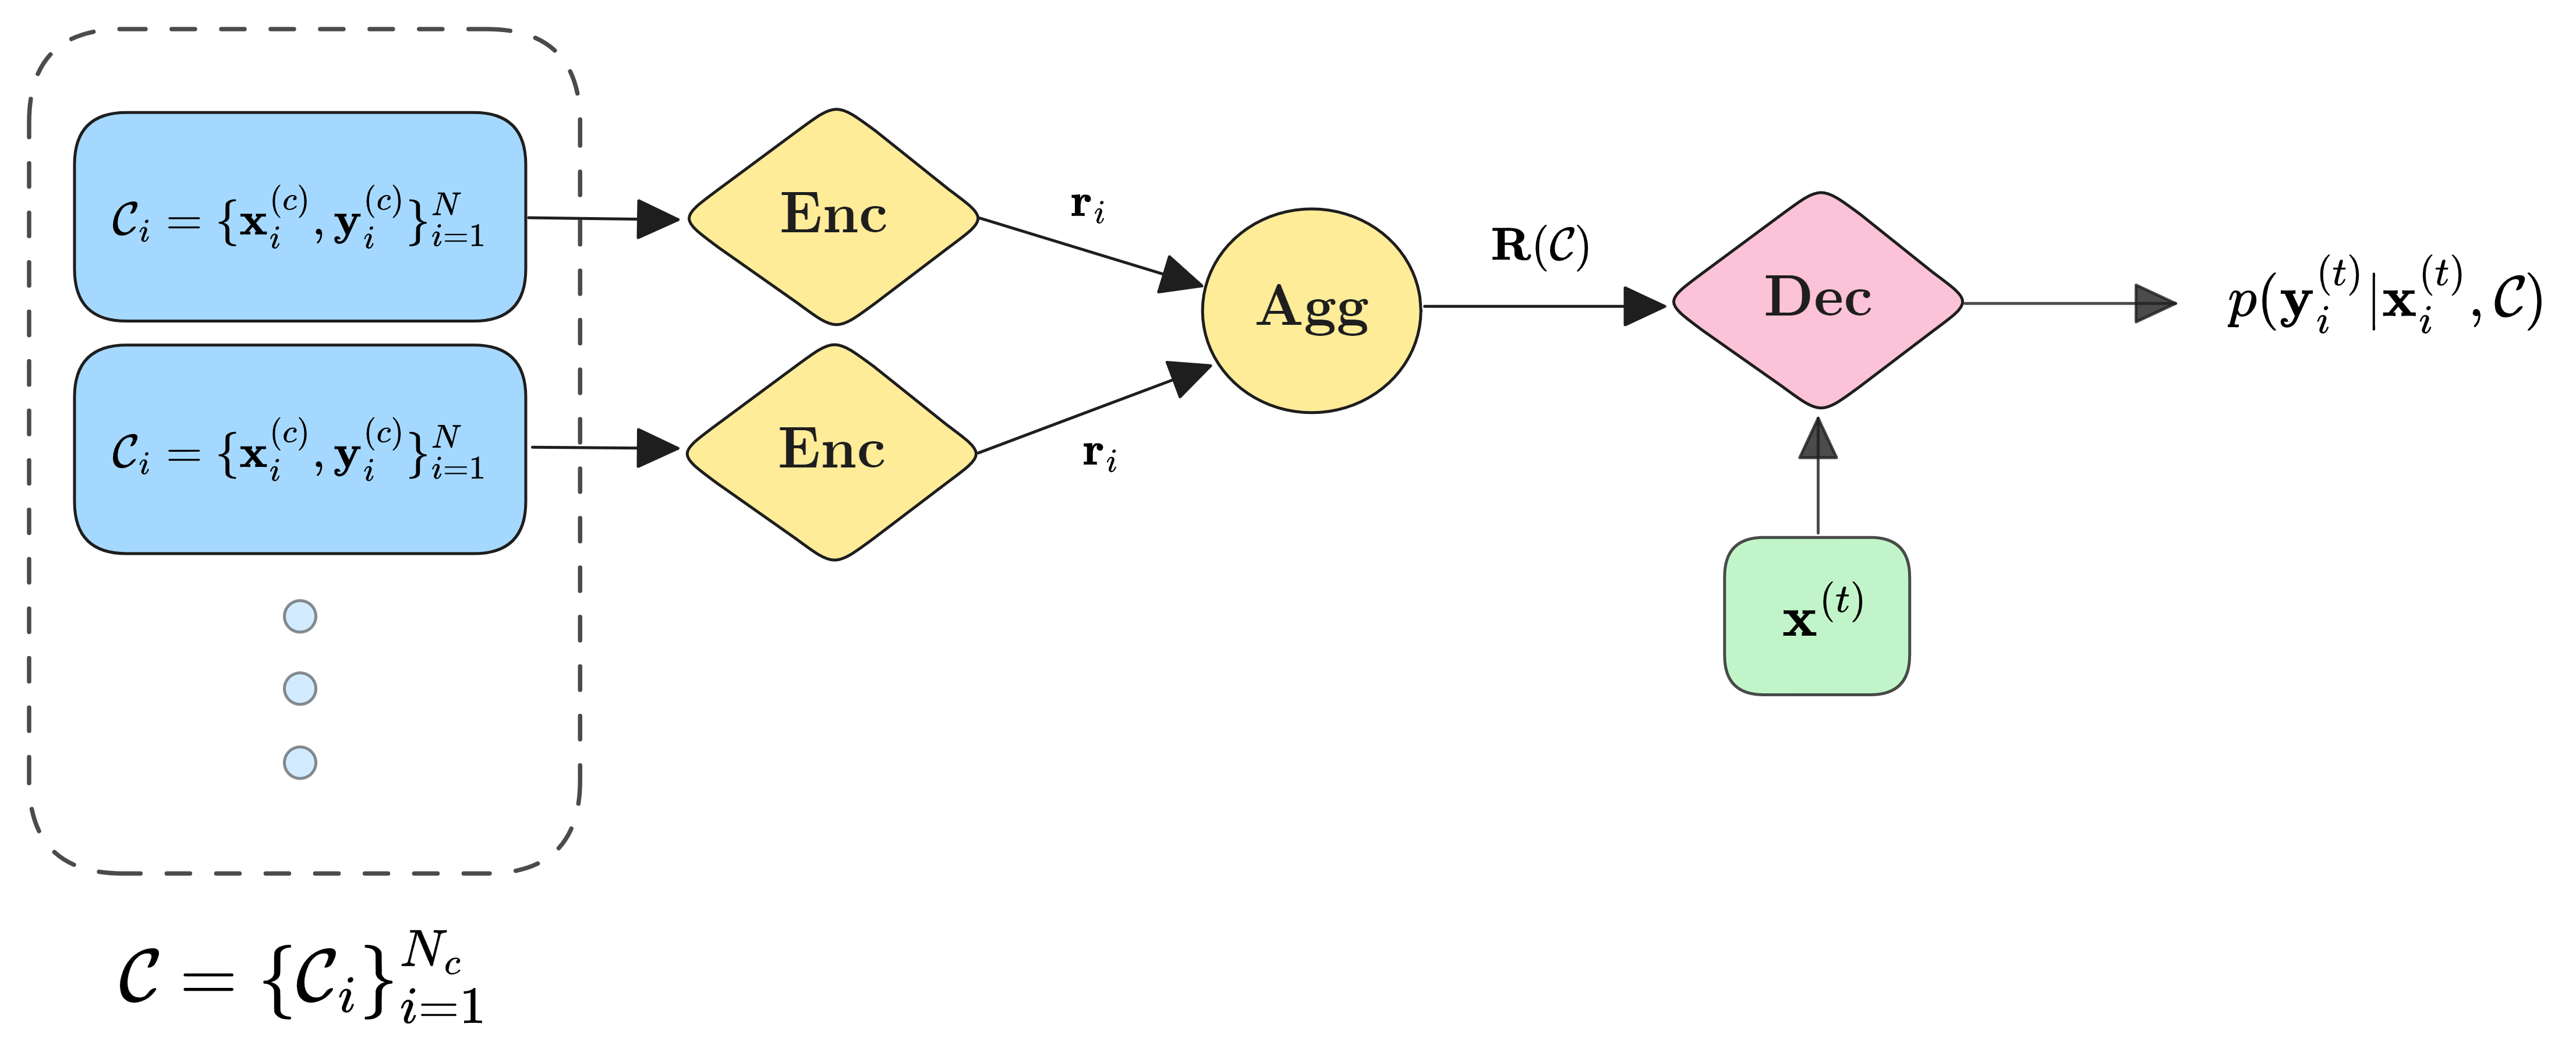
\includegraphics[height=0.3\textwidth]{./cnp.png}
	\caption{CNP Architecture: The model vectorizes each individual data point $\mathcal{C}_i$ in the context set $\mathcal{C}$ and then processes them to obtain a global representation $\bm{R}(\mathcal{C})$ which is then used to condition the decoder to predict a distribution over the target points $\bm{y}\isup{t}$.}
    \label{fig:cnp-architecture}
\end{figure}


In the original CNP paper, the encoder and decoder are implemented as simple Multi-Layer Perceptrons (MLPs) and the processing is implemented as a mean operation, which is an implementation of the `DeepSet' architecture \parencite{zaheer2018deep}.


Importantly, CNPs make the strong assumption that the posterior distribution \emph{factorizes} over the target points:

\begin{align}
    p(\bm{Y}\isup{t} | \bm{X}\isup{t}, \mathcal{C}) &\stackrel{(a)}{=} \prod_{i=1}^{N_t} p(\bm{{y}_i\isup{t}} | \bm{{x}_i\isup{t}}, \bm{R}(\mathcal{C})) \\ &\stackrel{(b)}{=} \prod_{i=1}^{N_t} \mathcal{N}(\bm{{y}_i\isup{t}} | \bm{\mu_i}, \bm{\sigma_i}^2) 
\end{align}

The  factorization assumption (a) allows the model can scale linearly with the number of target points with a tractable likelihood. However, this assumption means
\textbf{CNPs are unable to generate coherent sample paths, they are only able to produce distributions over the target points.} Furthermore, we need to select a marginal likelihood for the distribution (b) which is usually a Heteroscedastic Gaussian Likelihood (Gaussian with a variance that varies with the input) \parencite{garnelo2018conditional}. This adds an assumption since likelihood chosen may not be appropriate for the data we are modeling.

The model can be trained using simple maximum likelihood estimation (MLE) by minimizing the negative log-likelihood, giving us the following loss function:

\begin{equation}
    \mathcal{L} = \mathbb{E}_{(\mathcal{C}, \mathcal{T})} \left[- \sum_{i=1}^{|\mathcal{T}|} \log p(\bm{{y}_i\isup{t}} | \bm{{x}_i\isup{t}}, \mathcal{C})\right]
\end{equation}




\section{Performance of Vanilla NP}

Whilst the CNP using DeepSets is flexible and scalable, in reality it is unable to perform well on more complicated and higher dimensional data as the model is unable to learn a good representation of the data using a simple MLP and summation operation. 

\emph{Could we replace the encoder and decoder with more powerful networks? And if so, what would be the best architecture to use?} 

We aim to answer this by exploring the use of a Convolutional Neural Network (CNN) and a Transformer as encoders of our NP. CNNs and Transformers have been shown to perform well on a variety of tasks and at scale, thus we hypothesize that they will be able to learn a better representation of the context set and improve the performance of the NP.
Both are bound to have their unique advantages and disadvantages which we will explore in the following chapters.



% \ifSubfilesClassLoaded{%
%     \printbibliography{}
% }{} 


\end{document}